% MICRO 2026 Survey Paper - ML Performance Models
% Using MICRO 59 ACM sigconf template
% Last compiled: 2026-02-07 (rebuild triggered)

%%
%% For submission and review of your manuscript please change the
%% command to \documentclass[manuscript, screen, review]{acmart}.
%%
\documentclass[sigconf, screen, review]{acmart}

%%
%% \BibTeX command to typeset BibTeX logo in the docs
\AtBeginDocument{%
  \providecommand\BibTeX{{%
    Bib\TeX}}}

%% Rights management information - for submission
\setcopyright{none}
\copyrightyear{2026}
\acmYear{2026}
\acmDOI{}

%% Conference information
\acmConference[MICRO 2026]{The 59th IEEE/ACM International Symposium on Microarchitecture}{November 2026}{Austin, TX, USA}
\acmISBN{}

%% Disable ACM reference format printing for submission
\settopmatter{printfolios=true}
\settopmatter{printacmref=false}

%% Anonymous submission
\author{Anonymous Author(s)}
\affiliation{%
  \institution{Under Review}
  \country{Anonymous}
}

%% Additional packages (acmart already loads amsmath, amsfonts, amssymb, booktabs)
\usepackage{multirow}
\usepackage{tikz}
\usetikzlibrary{shapes.geometric,arrows.meta,positioning,fit,backgrounds,patterns}
\usepackage{pgfplots}
\pgfplotsset{compat=1.18}
\usepgfplotslibrary{groupplots}
\usetikzlibrary{plotmarks}

% Custom commands
\newcommand{\todo}[1]{\textcolor{red}{[TODO: #1]}}

\begin{document}

\title{A Survey of High-Level Modeling and Simulation Methods for Modern Machine Learning Workloads}
\subtitle{\normalsize{MICRO 2026 Submission -- Confidential Draft -- Do NOT Distribute!!}}

%%
%% The abstract is a short summary of the work to be presented in the
%% article.

%%%%%% -- PAPER CONTENT STARTS-- %%%%%%%%

\begin{abstract}
As machine learning workloads grow in scale and complexity---spanning training and inference for CNNs, transformers, mixture-of-experts models, and LLMs---architects and system designers need fast, accurate methods to predict their performance across diverse hardware platforms.
This survey provides a comprehensive analysis of the tools and methods available for modeling and simulating the performance of ML workloads, covering analytical models, cycle-accurate simulators, trace-driven approaches, and ML-augmented hybrid techniques.
We survey approximately 25 tools drawn from 53 papers across architecture venues (MICRO, ISCA, HPCA, ASPLOS) and systems venues (MLSys, OSDI, NSDI) published between 2016--2026, spanning DNN accelerator modeling (Timeloop, MAESTRO, Sparseloop), GPU simulation (GPGPU-Sim, Accel-Sim, NeuSight), distributed training simulation (ASTRA-sim, Lumos, SimAI), and LLM inference serving (VIDUR, Frontier, AMALI).
We organize the literature along three dimensions---methodology type (analytical, simulation, ML-augmented, hybrid), target platform (accelerators, GPUs, distributed systems, edge devices), and abstraction level (kernel, model, system)---while additionally characterizing tools by workload coverage, revealing a pervasive CNN-validation bias.
Our analysis reveals that hybrid approaches combining analytical structure with learned components achieve the best accuracy-speed trade-offs, while pure analytical models offer superior interpretability for design space exploration.
We conduct hands-on reproducibility evaluations of five representative tools, finding that reproducibility varies dramatically: Docker-first tools score 8.5+/10 on our rubric while tools relying on serialized ML models risk becoming unusable.
We identify key open challenges including cross-workload generalization beyond CNNs, composition of kernel-level predictions to end-to-end accuracy, and support for emerging architectures.
This survey provides practitioners guidance for selecting appropriate modeling tools and researchers a roadmap for advancing the field of ML workload performance prediction.
\end{abstract}

%%
%% Keywords
\keywords{ML workload performance prediction, DNN accelerator modeling, GPU simulation, distributed training simulation, LLM inference serving, design space exploration, survey}

\maketitle

% ==============================================================================
% INTRODUCTION
% ==============================================================================
\section{Introduction}
\label{sec:introduction}

Machine learning workloads---spanning training and inference for CNNs, transformers, mixture-of-experts models, and graph neural networks---have become the dominant consumers of compute across datacenters and edge devices.
The shift toward domain-specific architectures~\cite{hennessy2019golden}, from Google's TPU~\cite{tpuv1_2017,tpuv4_2023} to custom training accelerators, has created a heterogeneous hardware landscape where architects and system designers need fast, accurate performance predictions to navigate vast design spaces, select parallelization strategies, provision serving infrastructure, and optimize hardware-software co-design.
Yet ML workloads pose unique modeling challenges: they exhibit diverse computational patterns (dense matrix operations in attention layers, sparse accesses in GNNs, communication-bound collective operations in distributed training) across this increasingly heterogeneous landscape of GPUs, TPUs, custom accelerators, and multi-device clusters.

A rich ecosystem of tools has emerged, spanning analytical models (Timeloop~\cite{timeloop2019}, MAESTRO~\cite{maestro2019}: 5--10\% error at microsecond speed), cycle-accurate simulators (GPGPU-Sim~\cite{gpgpusim2009}, Accel-Sim~\cite{accelsim2020}: detailed but hours per workload), trace-driven simulators (ASTRA-sim~\cite{astrasim2023}, VIDUR~\cite{vidur2024}: system-scale training and serving), and ML-augmented hybrid approaches (NeuSight~\cite{neusight2025}: 2.3\% error on GPU kernels).
Each methodology occupies a distinct point in the accuracy-speed-generality trade-off space.

Despite this rich tool landscape, no comprehensive survey organizes these methods from the perspective of the ML workload practitioner---the architect or engineer who needs to select a modeling tool for a specific design or deployment task.
Existing surveys focus on ML \emph{techniques} for performance modeling~\cite{granite2022} or on specific hardware targets~\cite{timeloop2019}, leaving practitioners without guidance on which tools suit their needs across the full modeling spectrum.
This survey fills that gap by providing a methodology-centric view of the tools and methods available for predicting ML workload performance.

We make the following contributions:
\begin{itemize}
    \item A \textbf{methodology-centric taxonomy} organizing tools along three dimensions: methodology type (analytical, simulation, ML-augmented, hybrid), target platform (DNN accelerators, GPUs, distributed systems, edge devices), and abstraction level (kernel, model, system), with a quantitative coverage matrix identifying research gaps and a workload coverage analysis exposing the CNN-validation bias in the literature.
    \item A \textbf{systematic survey} of over 30 modeling tools drawn from 53 papers across architecture venues (MICRO, ISCA, HPCA, ASPLOS) and systems venues (MLSys, OSDI, NSDI) published between 2016--2026, using documented selection criteria.
    \item A \textbf{comparative analysis} examining trade-offs between accuracy, speed, generalization, and interpretability, with careful qualification of paper-reported accuracy claims and identification of cases where reported numbers are unverifiable.
    \item \textbf{Hands-on reproducibility evaluations} of representative tools with a 10-point rubric, and identification of \textbf{open challenges} including the CNN-to-transformer generalization gap, kernel-to-end-to-end error composition, and emerging accelerator support.
\end{itemize}

The paper proceeds as follows: Section~\ref{sec:methodology} describes our methodology; Section~\ref{sec:background} provides background; Section~\ref{sec:taxonomy} presents the taxonomy; Section~\ref{sec:survey} surveys tools by platform; Section~\ref{sec:comparison} compares accuracy and provides tool selection guidance; Section~\ref{sec:evaluation} presents reproducibility evaluations; Section~\ref{sec:challenges} discusses open challenges; and Section~\ref{sec:conclusion} concludes.

The field has evolved from early analytical frameworks (Eyeriss~\cite{eyeriss2016}, Paleo~\cite{paleo2017}) through systematic accelerator modeling (Timeloop~\cite{timeloop2019}, MAESTRO~\cite{maestro2019}) and distributed training simulation (ASTRA-sim~\cite{astrasim2020}), to modern hybrid analytical+learned approaches (NeuSight~\cite{neusight2025}) and LLM-specific modeling (VIDUR~\cite{vidur2024}, Frontier~\cite{frontier2025}); Table~\ref{tab:survey-summary} provides a comprehensive chronological overview.

% ==============================================================================
% SURVEY METHODOLOGY
% ==============================================================================
\section{Survey Methodology}
\label{sec:methodology}

We searched ACM Digital Library, IEEE Xplore, Semantic Scholar, and arXiv using terms related to ML performance modeling, with backward/forward citation tracking from seminal works.
Target venues include architecture (MICRO, ISCA, HPCA, ASPLOS), systems (MLSys, OSDI, SOSP, NSDI), and related (NeurIPS, MobiSys, DAC, ISPASS).
Papers must propose or evaluate a tool for predicting ML workload performance with quantitative evaluation; we exclude non-performance tasks and general-purpose workloads.
From 287 initial candidates, title/abstract screening yielded 118 papers; full-text review reduced the set to 53 that met all criteria, supplemented by 12 foundational works for context.
We cover 2016--2026 and classify each paper by \emph{methodology type} (analytical, simulation, trace-driven, ML-augmented, hybrid), \emph{target platform}, and \emph{abstraction level} (kernel, model, system).

\subsection{Related Surveys}
\label{subsec:related-surveys}

Prior surveys address adjacent topics: Rakhshanfar and Zarandi~\cite{rakhshanfar2021survey} survey ML for processor DSE; Sze et al.~\cite{sze2017efficient} treat DNN hardware design (the foundation for Timeloop/MAESTRO); GPGPU-Sim~\cite{gpgpusim2009} and gem5~\cite{binkert2011gem5} have extensive evaluation literature; and MLPerf~\cite{mlperf_training2020,mlperf_inference2020} standardizes \emph{measurement} rather than \emph{prediction}.
This survey differs by spanning the full methodology spectrum across all major platforms with hands-on reproducibility evaluations.
The closest prior work, Dudziak et al.~\cite{latencypredictorsnas2024}, compares edge device predictors for NAS; we broaden to the full landscape.

% ==============================================================================
% BACKGROUND
% ==============================================================================
\section{Background}
\label{sec:background}

\subsection{ML Workload Characteristics}
\label{subsec:workload-characteristics}

ML workloads, defined as computation graphs in frameworks like PyTorch~\cite{pytorch2019} and TensorFlow~\cite{tensorflow2016}, present distinct modeling challenges.
Their operators (convolutions, matrix multiplications, attention) have statically known shapes amenable to analytical modeling, though mixture-of-experts and dynamic inference introduce input-dependent control flow.
Performance is highly sensitive to how tensors map onto specialized memory hierarchies (dataflow, tiling, loop ordering), and for LLM inference, KV cache management dominates memory behavior~\cite{vllm2023}.
At scale, training distributes across thousands of GPUs via data, tensor, pipeline, and expert parallelism~\cite{llama3scaling2025}, requiring system-level modeling of compute--memory--network interactions.
LLM inference further splits into compute-bound prefill and memory-bound decode phases~\cite{splitwise2024}, both of which must be modeled under batched serving~\cite{sarathi2024,orca2022}.

\subsection{Modeling Methodologies}
\label{subsec:modeling-methodologies}

We classify approaches into four categories forming our taxonomy's primary axis.
\textbf{Analytical models} express performance as closed-form functions---e.g., the roofline model~\cite{williams2009roofline} bounds throughput by $P = \min(\pi, \beta \cdot I)$, while Timeloop~\cite{timeloop2019} computes data movement costs for DNN accelerator mappings. They offer microsecond evaluation but require per-architecture derivation.
\textbf{Cycle-accurate simulators} (gem5~\cite{binkert2011gem5}, GPGPU-Sim~\cite{gpgpusim2009}, Accel-Sim~\cite{accelsim2020}) achieve high fidelity but at $1000$--$10000\times$ slowdown; sampling techniques~\cite{simpoint2002,smarts2003} help but were not designed for ML workloads.
\textbf{Trace-driven simulators} like ASTRA-sim~\cite{astrasim2023} (distributed training via Chakra traces~\cite{chakra2023}) and VIDUR~\cite{vidur2024} (LLM serving) trade some fidelity for orders-of-magnitude speedup.
\textbf{ML-augmented approaches} learn performance functions from profiling data, ranging from random forests (nn-Meter~\cite{nnmeter2021}) and XGBoost (TVM~\cite{tvm2018}) to deep learning (NeuSight~\cite{neusight2025}) and meta-learning (HELP~\cite{help2021}); they capture non-linear relationships but may not generalize beyond their training distribution.

\subsection{Problem Formulation}
\label{subsec:problem-formulation}

Performance modeling maps workload $\mathcal{W}$ and hardware $\mathcal{H}$ to a metric $y$: $\hat{y} = f(\mathcal{W}, \mathcal{H}; \theta)$, with workloads represented at operator, graph, IR, or trace level, and hardware characterized by specifications, counters, or learned embeddings.
Prediction targets include latency, throughput, energy, and memory footprint.
Accuracy metrics---MAPE, RMSE, and rank correlation (Kendall's $\tau$)---vary across the literature, and differences in benchmarks, hardware targets, and evaluation protocols limit direct comparison (Section~\ref{sec:comparison}).

% ==============================================================================
% TAXONOMY
% ==============================================================================
\section{Taxonomy}
\label{sec:taxonomy}

We organize the literature along three dimensions.
The \emph{primary axis} is methodology type---how a tool predicts performance---because methodology determines the fundamental trade-offs between accuracy, speed, interpretability, and data requirements.
The \emph{secondary axes} are target platform and abstraction level, which together determine the scope and applicability of each tool.
We additionally characterize tools by workload coverage, exposing a pervasive CNN-validation bias in the literature.

Table~\ref{tab:taxonomy-matrix} provides a unified view combining the coverage matrix (number of surveyed tools per methodology--platform cell) with trade-off profiles, with empty cells highlighting research gaps.
The dominant pairings are: analytical models for accelerators, cycle-accurate simulation for GPUs/CPUs, trace-driven simulation for distributed systems, and ML-augmented approaches for edge devices.

% --- Unified Taxonomy Table (merged from Tables 1+2, issue #192) ---
\begin{table*}[t]
\centering
\caption{Methodology taxonomy: coverage matrix and trade-off profile.
Platform columns show the number of surveyed tools per cell; \textbf{0} indicates an explicit research gap.
Speed, data requirements, and interpretability determine practical applicability; the failure mode column identifies the primary condition under which each methodology breaks down.}
\label{tab:taxonomy-matrix}
\small
\begin{tabular}{l|ccccc|cccc}
\toprule
 & \textbf{DNN} & & \textbf{Distrib.} & \textbf{Edge/} & & \textbf{Eval.} & \textbf{Data} & & \textbf{Failure} \\
\textbf{Methodology} & \textbf{Accel.} & \textbf{GPU} & \textbf{Systems} & \textbf{Mobile} & \textbf{CPU} & \textbf{Speed} & \textbf{Req.} & \textbf{Interp.} & \textbf{Mode} \\
\midrule
Analytical       & 3 & 3 & 2 & \textbf{0} & \textbf{0} & $\mu$s & None & High & Dynamic effects \\
Cycle-Accurate   & 1 & 2 & \textbf{0} & \textbf{0} & 1 & Hours & Binary & High & Scale \\
Trace-Driven     & \textbf{0} & \textbf{0} & 7 & \textbf{0} & \textbf{0} & Min. & Traces & Med. & Trace fidelity \\
ML-Augmented     & \textbf{0} & 3 & \textbf{0} & 3 & 1 & ms & Profiling & Low & Distrib.\ shift \\
Hybrid           & 1 & 2 & \textbf{0} & \textbf{0} & 1 & ms & Mixed & Med. & Training domain \\
\bottomrule
\end{tabular}
\end{table*}

Table~\ref{tab:taxonomy-matrix} reveals three structural observations.
First, trace-driven simulation is exclusively used for distributed systems---no surveyed tool applies trace-driven methods to single-device GPU or accelerator modeling, despite the potential for trace-driven approaches to avoid the slowdown of cycle-accurate simulation while retaining more fidelity than analytical models.
Second, edge/mobile devices are served exclusively by ML-augmented approaches; the absence of analytical or hybrid models for edge devices reflects the hardware diversity problem but also represents a research gap, since hybrid approaches could combine the interpretability of analytical models with the adaptability of learned components.
Third, no ML-augmented or hybrid tool specifically targets distributed system modeling---tools like VIDUR use ML internally for kernel prediction but are architecturally trace-driven simulators.
The trade-off columns further show that methodologies cluster into two speed regimes: sub-millisecond (analytical, ML-augmented, hybrid) suitable for design space exploration, and minutes-to-hours (simulation, trace-driven) suitable for detailed validation.

\subsection{Primary Axis: Methodology Type}
\label{subsec:by-methodology}

The choice of methodology determines fundamental trade-offs (Table~\ref{tab:taxonomy-matrix}); Section~\ref{sec:survey} provides detailed per-tool analysis.
\textbf{Analytical models} express performance as closed-form functions, offering microsecond evaluation and full interpretability but requiring per-architecture derivation (e.g., Timeloop~\cite{timeloop2019}: 5--10\% error at 2000$\times$ speedup).
\textbf{Cycle-accurate simulators} (GPGPU-Sim~\cite{gpgpusim2009}, Accel-Sim~\cite{accelsim2020}) achieve high fidelity at $1000$--$10000\times$ slowdown, impractical for DSE.
\textbf{Trace-driven simulators} replay execution traces for system-level modeling (ASTRA-sim~\cite{astrasim2023}: 5--15\% error; VIDUR~\cite{vidur2024}: $<$5\%), with some using ML internally.
\textbf{ML-augmented models} learn from profiling data (nn-Meter~\cite{nnmeter2021}, TVM~\cite{tvm2018}), but suffer from \emph{silent distribution shift}.
\textbf{Hybrid} approaches combine analytical structure with learned residuals (NeuSight~\cite{neusight2025}: 2.3\% MAPE), achieving the best accuracy--speed trade-offs; transfer learning provides 22.5\% average improvement~\cite{latencypredictorsnas2024}.

\subsection{Secondary Axes: Platform and Abstraction Level}
\label{subsec:by-platform}

The target platform constrains applicable methodologies: \textbf{DNN accelerators}~\cite{tpuv1_2017,tpuv4_2023} are best served by analytical models (Timeloop, MAESTRO, Sparseloop) due to regular memory hierarchies; \textbf{GPUs} span the full methodology spectrum reflecting SIMT complexity; \textbf{distributed systems} require trace-driven simulation (ASTRA-sim, VIDUR, SimAI) for collective communication and pipeline parallelism; \textbf{edge/mobile devices} are dominated by ML-augmented approaches (nn-Meter, LitePred, HELP) due to hardware diversity; and \textbf{CPUs} are less studied for ML workloads (Concorde~\cite{concorde2025}, GRANITE~\cite{granite2022}).

Abstraction level determines where composition errors arise.
\textbf{Kernel-level} tools (NeuSight, nn-Meter, TVM) achieve 2--3\% error but composing predictions into end-to-end latency introduces errors from memory allocation, kernel launch overhead, and inter-operator data movement.
\textbf{Model-level} tools (Paleo, Habitat, AMALI) account for graph-level effects at 5--12\% error.
\textbf{System-level} tools (ASTRA-sim, VIDUR, SimAI) capture communication and scheduling at 5--15\% error, with kernel-level errors propagating through the composition chain.
Figure~\ref{fig:abstraction-levels} illustrates this hierarchy.

\begin{figure}[t]
\centering
\resizebox{\columnwidth}{!}{%
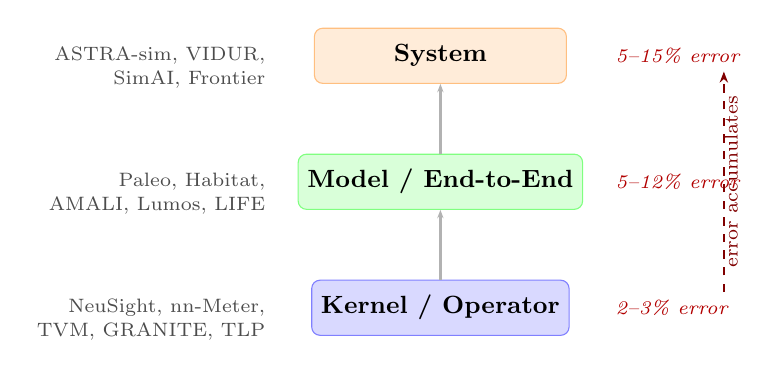
\begin{tikzpicture}[
  level/.style={draw, rounded corners=3pt, minimum width=3.2cm, minimum height=0.7cm, align=center, font=\small\bfseries},
  tool/.style={font=\scriptsize, text=black!70},
  err/.style={font=\scriptsize\itshape, text=red!70!black},
  arrow/.style={-{Stealth[length=3pt]}, thick, gray!60},
  compos/.style={-{Stealth[length=4pt]}, thick, red!50!black, dashed},
]

% Levels (bottom to top)
\node[level, fill=blue!15, draw=blue!50] (kernel) at (0,0) {Kernel / Operator};
\node[level, fill=green!15, draw=green!50] (model) at (0,1.6) {Model / End-to-End};
\node[level, fill=orange!15, draw=orange!50] (system) at (0,3.2) {System};

% Composition arrows between levels
\draw[arrow] (kernel) -- (model);
\draw[arrow] (model) -- (system);

% Tool names (left side)
\node[tool, anchor=east] at (-2.1,0) {NeuSight, nn-Meter,};
\node[tool, anchor=east] at (-2.1,-0.3) {TVM, GRANITE, TLP};
\node[tool, anchor=east] at (-2.1,1.6) {Paleo, Habitat,};
\node[tool, anchor=east] at (-2.1,1.3) {AMALI, Lumos, LIFE};
\node[tool, anchor=east] at (-2.1,3.2) {ASTRA-sim, VIDUR,};
\node[tool, anchor=east] at (-2.1,2.9) {SimAI, Frontier};

% Error ranges (right side)
\node[err, anchor=west] at (2.1,0) {2--3\% error};
\node[err, anchor=west] at (2.1,1.6) {5--12\% error};
\node[err, anchor=west] at (2.1,3.2) {5--15\% error};

% Composition problem annotation
\draw[compos] (3.6,0.2) -- (3.6,3.0);
\node[font=\scriptsize, text=red!50!black, rotate=90, anchor=south] at (3.9,1.6) {error accumulates};

\end{tikzpicture}%
}
\caption{Abstraction level hierarchy and the composition problem. Tools operate at one of three levels; composing predictions across levels accumulates error. Error ranges are representative values from surveyed papers.}
\label{fig:abstraction-levels}
\end{figure}

\subsection{Workload Coverage}
\label{subsec:workload-coverage}

Table~\ref{tab:workload-coverage} characterizes the workload types on which each tool has been validated, exposing a pervasive CNN-validation bias.

\begin{table}[t]
\centering
\caption{Workload validation coverage. \checkmark\ = validated in the original paper; $\circ$ = partial or indirect validation; --- = no validation.
Nearly all tools report accuracy on CNN workloads; transformer and MoE coverage is sparse.
Empty columns (diffusion, dynamic inference) represent workload types with \emph{no} validated performance modeling tools.}
\label{tab:workload-coverage}
\small
\begin{tabular}{lccccc}
\toprule
 & & \textbf{Trans-} & \textbf{LLM} & & \\
\textbf{Tool} & \textbf{CNN} & \textbf{former} & \textbf{Train} & \textbf{MoE} & \textbf{Diff.} \\
\midrule
Timeloop & \checkmark & $\circ$ & --- & --- & --- \\
MAESTRO & \checkmark & --- & --- & --- & --- \\
NeuSight & \checkmark & \checkmark & --- & --- & --- \\
Habitat & \checkmark & --- & --- & --- & --- \\
AMALI & --- & \checkmark & --- & --- & --- \\
ASTRA-sim & \checkmark & $\circ$ & \checkmark & --- & --- \\
VIDUR & --- & \checkmark & --- & --- & --- \\
SimAI & --- & --- & \checkmark & --- & --- \\
Lumos & --- & --- & \checkmark & --- & --- \\
Frontier & --- & \checkmark & --- & \checkmark & --- \\
nn-Meter & \checkmark & --- & --- & --- & --- \\
LitePred & \checkmark & --- & --- & --- & --- \\
HELP & \checkmark & --- & --- & --- & --- \\
TVM/Ansor & \checkmark & $\circ$ & --- & --- & --- \\
\bottomrule
\end{tabular}
\end{table}

The table reveals that \textbf{no surveyed tool has been validated on diffusion models or dynamic inference workloads}~\cite{dynamicreasoning2026}, only Frontier~\cite{frontier2025} has validated MoE support, and no single tool offers validated transformer prediction across the full kernel-to-system stack.
Practitioners working with non-CNN workloads must accept unvalidated predictions, collect their own validation data, or fall back to measurement.

% ==============================================================================
% SURVEY OF APPROACHES
% ==============================================================================
\section{Survey of Approaches}
\label{sec:survey}

This section surveys performance modeling tools for ML workloads, organized by target platform, examining modeling challenges, available tools, and their strengths and limitations.
Table~\ref{tab:survey-summary} provides a comprehensive comparison.

\begin{table*}[t]
\centering
\caption{Summary of surveyed performance modeling tools for ML workloads, organized by target platform. \textbf{Methodology}: A=Analytical, S=Simulation, T=Trace-driven, M=ML-augmented, H=Hybrid. $^*$Accuracy measures surrogate-vs-simulator fidelity, not real hardware error. $^\dagger$Reported accuracy unverifiable due to reproducibility issues. $^\ddagger$No accuracy baseline against real hardware reported.}
\label{tab:survey-summary}
\small
\begin{tabular}{lllllll}
\toprule
\textbf{Tool} & \textbf{Platform} & \textbf{Method} & \textbf{Target} & \textbf{Accuracy} & \textbf{Speed} & \textbf{Key Capability} \\
\midrule
\multicolumn{7}{l}{\textit{DNN Accelerator Modeling}} \\
Timeloop~\cite{timeloop2019} & NPU & A & Latency/Energy & 5--10\% & $\mu$s & Loop-nest DSE \\
MAESTRO~\cite{maestro2019} & NPU & A & Latency/Energy & 5--15\% & $\mu$s & Data-centric directives \\
Sparseloop~\cite{sparseloop2022} & NPU & A & Sparse tensors & 5--10\% & $\mu$s & Compression modeling \\
PyTorchSim~\cite{pytorchsim2025} & NPU & S & Cycle-accurate & N/A$^\ddagger$ & Hours & PyTorch 2 integration \\
ArchGym~\cite{archgym2023} & Multi & H & Multi-objective & 0.61\%$^*$ & ms & ML-aided DSE \\
\midrule
\multicolumn{7}{l}{\textit{GPU Performance Modeling}} \\
Accel-Sim~\cite{accelsim2020} & GPU & S & Cycle-accurate & 10--20\% & Hours & SASS trace-driven \\
GPGPU-Sim~\cite{gpgpusim2009} & GPU & S & Cycle-accurate & 10--20\% & Hours & CUDA workloads \\
AMALI~\cite{amali2025} & GPU & A & LLM inference & 23.6\% & ms & Memory hierarchy \\
NeuSight~\cite{neusight2025} & GPU & H & Kernel/E2E latency & 2.3\% & ms & Tile-based prediction \\
Habitat~\cite{habitat2021} & GPU & H & Training time & 11.8\% & Per-kernel & Wave scaling \\
\midrule
\multicolumn{7}{l}{\textit{Distributed Training and LLM Serving}} \\
ASTRA-sim~\cite{astrasim2023} & Distributed & T & Training time & 5--15\% & Minutes & Collective modeling \\
SimAI~\cite{simai2025} & Distributed & T & Training time & 1.9\% & Minutes & Full-stack simulation \\
Lumos~\cite{lumos2025} & Distributed & T & LLM training & 3.3\% & Minutes & H100 training \\
VIDUR~\cite{vidur2024} & GPU cluster & T & LLM serving & $<$5\% & Seconds & Prefill/decode phases \\
Frontier~\cite{frontier2025} & Distributed & T & MoE inference & --- & Minutes & Stage-centric sim. \\
TrioSim~\cite{triosim2025} & Multi-GPU & T & DNN training & N/A$^\ddagger$ & Minutes & Lightweight multi-GPU \\
\midrule
\multicolumn{7}{l}{\textit{Edge Device Modeling}} \\
nn-Meter~\cite{nnmeter2021} & Edge & M & Latency & $<$1\%$^\dagger$ & ms & Kernel detection \\
LitePred~\cite{litepred2024} & Edge & M & Latency & 0.7\% & ms & 85-platform transfer \\
HELP~\cite{help2021} & Multi & M & Latency & 1.9\% & ms & 10-sample adaptation \\
\midrule
\multicolumn{7}{l}{\textit{Compiler Cost Models}} \\
TVM~\cite{tvm2018} & GPU & M & Schedule perf. & $\sim$15\% & ms & Autotuning guidance \\
Ansor~\cite{ansor2020} & GPU & M & Schedule perf. & $\sim$15\% & ms & Program sampling \\
TLP~\cite{tlp2023} & GPU & M & Tensor program & $<$10\% & ms & Transformer cost model \\
\bottomrule
\end{tabular}
\end{table*}

\subsection{DNN Accelerator Modeling}
\label{subsec:accelerator-modeling}

DNN accelerators employ specialized dataflows and memory hierarchies optimized for tensor operations~\cite{sze2017efficient}, and their computational regularity makes this domain particularly amenable to analytical modeling.

\textbf{Analytical frameworks} dominate.
Timeloop~\cite{timeloop2019} computes data reuse, latency, and energy from loop-nest representations at 5--10\% error versus RTL simulation with 2000$\times$ speedup, and provides deterministic reference outputs for standard designs (Eyeriss~\cite{eyeriss2016}, Simba).
MAESTRO~\cite{maestro2019} simplifies specification via data-centric directives but is less precise for energy modeling.
Sparseloop~\cite{sparseloop2022} extends Timeloop to sparse tensors by modeling sparsity patterns, compression formats (CSR, bitmap), and hardware intersection units---critical for transformer inference but limited to static, known sparsity distributions.

\textbf{Simulation and ML-augmented approaches.}
PyTorchSim~\cite{pytorchsim2025} integrates PyTorch~2 with cycle-accurate NPU simulation, directly consuming computation graphs to eliminate manual workload translation, but does not report real-hardware accuracy and inherits simulation speed limitations.
ArchGym~\cite{archgym2023} connects ML surrogates to analytical simulators for design space exploration; its 0.61\% RMSE measures surrogate-vs-simulator fidelity, not real-hardware accuracy.
\textbf{Synthesis.}
Accelerator modeling is the most mature subdomain, with Timeloop as the de facto DSE standard.
The key gap is silicon validation---no surveyed accelerator tool validates against manufactured hardware, leaving all anchored to RTL comparisons.
Emerging PIM modeling tools~\cite{upimulator2024,attacc2024,neupims2024,paise2025} lack real hardware validation (Section~\ref{sec:challenges}).

\subsection{GPU Performance Modeling}
\label{subsec:gpu-modeling}

GPUs dominate ML training and inference, requiring models that account for SIMT execution, warp scheduling, memory coalescing, and occupancy effects.

\textbf{Cycle-accurate simulation.}
GPGPU-Sim~\cite{gpgpusim2009} and Accel-Sim~\cite{accelsim2020} achieve 0.90--0.97 IPC correlation; recent reverse-engineering of modern GPU cores~\cite{dissectinggpu2025} improved Accel-Sim to 13.98\% MAPE.
However, $1000$--$10000\times$ slowdown makes these tools impractical at production scale.

\textbf{Analytical models.}
The roofline model~\cite{williams2009roofline} provides upper bounds but misses dynamic effects; Roofline-LLM~\cite{rooflinellm2024} extends it to LLM inference.
AMALI~\cite{amali2025} reduces LLM inference MAPE from 127\% to 23.6\% via memory hierarchy modeling---the residual error reflects the fundamental difficulty of analytically capturing GPU dynamic behavior (warp scheduling, cache contention).

\textbf{Hybrid learned models.}
NeuSight~\cite{neusight2025} achieves 2.3\% MAPE on GPT-3 inference (H100/A100/V100) via tile-based prediction mirroring CUDA execution.
Habitat~\cite{habitat2021} uses wave scaling to decompose compute and memory components, achieving 11.8\% cross-GPU transfer error (e.g., V100$\rightarrow$A100), but requires source GPU profiling and assumes occupancy patterns remain similar across generations.
Direct comparison requires caution: NeuSight targets 2023--2025 hardware with LLMs, while Habitat was designed for earlier GPUs with CNNs.

\textbf{LLM-specific modeling.}
LLM execution exhibits distinct prefill (compute-bound) and decode (memory-bound) phases~\cite{splitwise2024,distserve2024}.
VIDUR~\cite{vidur2024} simulates serving with scheduling strategies (Orca~\cite{orca2022}, Sarathi~\cite{sarathi2024}) at $<$5\% error; LIFE~\cite{life2025} and HERMES~\cite{hermes2025} target analytical and disaggregated inference, respectively.

\textbf{Compiler cost models.}
TVM~\cite{tvm2018} and Ansor~\cite{ansor2020} use ML cost models for autotuning at $\sim$15\% MAPE; TLP~\cite{tlp2023} uses transformer-based modeling at $<$10\% MAPE.
SynPerf~\cite{synperf2025} and SwizzlePerf~\cite{swizzleperf2025} prioritize ranking accuracy over absolute error.

\textbf{Synthesis.}
GPU modeling spans the widest methodological range (2\%--24\% error), reflecting the tension between microarchitectural complexity and rapid hardware evolution.
NeuSight offers the best accuracy--speed trade-off for LLM workloads, while AMALI and LIFE fill the pre-silicon gap despite higher error.

\subsection{Distributed Training and LLM Serving}
\label{subsec:distributed-modeling}

Distributed systems introduce communication overhead, synchronization barriers, and parallelism strategy choices across tensor~\cite{megatronlm2020}, pipeline~\cite{gpipe2019}, and data parallelism~\cite{zero2020}.

\textbf{Training simulation.}
ASTRA-sim~\cite{astrasim2023} provides end-to-end simulation via Chakra traces~\cite{chakra2023} at 5--15\% error versus HGX-H100 clusters.
SimAI~\cite{simai2025} achieves 1.9\% MAPE at Alibaba Cloud scale; Lumos~\cite{lumos2025} achieves 3.3\% on H100 training; TrioSim~\cite{triosim2025} and Echo~\cite{echo2024} offer additional approaches.
PRISM~\cite{prism2025} produces prediction intervals at 10K+ GPU scale.

\textbf{Scaling and parallelism.}
Paleo~\cite{paleo2017} pioneered analytical training-time estimation; MAD Max~\cite{madmax2024} extends this per parallelism dimension; Sailor~\cite{sailor2025} addresses heterogeneous clusters.
The Llama~3 study~\cite{llama3scaling2025} documents 4D parallelism at 16K H100 GPUs as validation ground truth.

\textbf{Inference serving.}
VIDUR~\cite{vidur2024} extends to distributed serving with vLLM~\cite{vllm2023} scheduling; Frontier~\cite{frontier2025} targets MoE and disaggregated inference; ThrottLL'eM~\cite{throttllem2025} models GPU power effects.
KV cache management remains the key bottleneck~\cite{vllm2023}, and algorithmic innovations (speculative decoding~\cite{medusa2024}) create a moving-target challenge for simulators.

\textbf{Synthesis.}
Distributed modeling is the fastest-growing subdomain, bifurcating into \emph{trace-driven fidelity} (ASTRA-sim, SimAI) and \emph{analytical decomposition} (Paleo, MAD Max), with PRISM's probabilistic approach as an emerging third path.

\subsection{Edge Device Modeling}
\label{subsec:edge-modeling}

Edge devices impose strict power, memory, and latency constraints, and their hardware diversity (mobile CPUs, GPUs, NPUs, DSPs) makes per-device analytical modeling impractical, driving ML-augmented approaches.

nn-Meter~\cite{nnmeter2021} reports $<$1\% MAPE but scores 3/10 in our reproducibility evaluation (Section~\ref{sec:evaluation}) due to unpinned dependencies.
LitePred~\cite{litepred2024} achieves 0.7\% MAPE across 85 (predominantly ARM) platforms; HELP~\cite{help2021} achieves 1.9\% via 10-sample meta-learning adaptation.
ESM~\cite{esm2025} finds well-tuned random forests match deep learning surrogates, and transfer learning provides 22.5\% average improvement~\cite{latencypredictorsnas2024}.

\textbf{Synthesis.}
Edge modeling is dominated by ML-augmented approaches with data quality and tool longevity mattering more than model sophistication---nn-Meter's reproducibility failure (Section~\ref{sec:evaluation}) underscores this lesson.

\subsection{Cross-Cutting Themes}
\label{subsec:cross-cutting}

\emph{Structural decomposition} mirroring hardware execution outperforms black-box approaches (Timeloop's loop nests, NeuSight's tiles, VIDUR's prefill/decode), while \emph{verifiable moderate accuracy} matters more than unverifiable high accuracy (Docker-first tools: 8.5+/10 vs.\ nn-Meter: 3/10).
A persistent \textbf{accuracy--generality--speed trilemma} explains why no single methodology dominates: each maximizes a different vertex at the expense of the others.

% ==============================================================================
% COMPARISON AND ANALYSIS
% ==============================================================================
\section{Comparison and Analysis}
\label{sec:comparison}

We analyze trade-offs across methodology types along accuracy and speed dimensions (see Table~\ref{tab:survey-summary} for per-tool details); generalization and interpretability challenges are deferred to Section~\ref{sec:challenges}.

\subsection{Accuracy by Problem Difficulty}
\label{subsec:accuracy-difficulty}

We organize accuracy results by inherent problem difficulty rather than comparing across incompatible benchmarks (see Table~\ref{tab:survey-summary} for per-tool accuracy).
Accelerator dataflow modeling is most tractable (Timeloop: 5--10\%); single-GPU kernel prediction achieves 2--12\% via hybrid methods (NeuSight, Habitat); distributed systems reach 2--15\% (SimAI 1.9\%, ASTRA-sim 5--15\%); cross-platform edge prediction achieves 0.7--2\% but requires per-device profiling; and GPU analytical modeling remains hardest (AMALI: 23.6\%).
Setup costs vary dramatically: analytical models require only architecture specifications, ML-augmented approaches need 10--10K profiling samples per device, and cycle-accurate simulators require hardware-specific binaries or traces.

\subsection{Practitioner Tool Selection}
\label{subsec:tool-selection}

Tool selection follows platform and use case.
For \emph{accelerator DSE}, use Timeloop or MAESTRO for microsecond-speed exhaustive search with interpretable bottleneck feedback.
For \emph{GPU evaluation}, NeuSight offers the best accuracy--speed balance for LLMs; use Accel-Sim when microarchitectural detail is needed.
For \emph{distributed systems}, use VIDUR for LLM serving configuration and ASTRA-sim or SimAI for training parallelism at scale.
For \emph{edge devices}, LitePred offers the broadest platform coverage, while HELP excels with minimal profiling data.

% ==============================================================================
% EXPERIMENTAL EVALUATION
% ==============================================================================
\section{Experimental Evaluation}
\label{sec:evaluation}

We conducted hands-on evaluations of five tools spanning methodology types: Timeloop (analytical), ASTRA-sim (trace-driven, distributed), VIDUR (trace-driven, LLM serving), nn-Meter (ML-augmented, edge), and NeuSight (hybrid, GPU).

\textbf{Environment and rubric.}
All evaluations ran on Apple M2 Ultra (aarch64, 192\,GB RAM) using Docker containers where provided---no GPU hardware was available, so we cannot validate absolute accuracy claims.
We score each tool on a 10-point rubric: \emph{Setup} (3 pts), \emph{Reproducibility} (4 pts), \emph{Usability} (3 pts).
Table~\ref{tab:evaluation-summary} summarizes results.

\begin{table}[t]
\centering
\caption{Reproducibility evaluation scores (10-point rubric). Tools are ranked by total score. $^\dagger$Timeloop CLI works but Python bindings fail.}
\label{tab:evaluation-summary}
\small
\begin{tabular}{lcccc}
\toprule
\textbf{Tool} & \textbf{Setup} & \textbf{Reprod.} & \textbf{Usability} & \textbf{Total} \\
\midrule
VIDUR & 2.5 & 3.5 & 3 & 9/10 \\
Timeloop$^\dagger$ & 3 & 4 & 2 & 9/10 \\
ASTRA-sim & 2.5 & 3 & 3 & 8.5/10 \\
NeuSight & 2 & 3 & 2.5 & 7.5/10 \\
nn-Meter & 2 & 0 & 1 & 3/10 \\
\bottomrule
\end{tabular}
\end{table}

\subsection{Per-Tool Results}
\label{subsec:per-tool-results}

\textbf{VIDUR} (9/10)---the highest-scoring tool.
We simulated Llama-2-7B inference on a simulated A100 using vLLM and Sarathi scheduling (Table~\ref{tab:vidur-results}).
VIDUR correctly captures scheduling trade-offs: Sarathi achieves 12.2\% lower latency than vLLM (0.158\,s vs.\ 0.177\,s) via chunked prefill~\cite{sarathi2024}, TPOT differs by only 3.5\% (confirming hardware-bound decode), and vLLM preempted 26.5\% of requests while Sarathi preempted zero---matching the algorithmic difference in KV-cache management~\cite{vllm2023}.
VIDUR's Docker-pinned dependencies avoid the serialization failures seen in nn-Meter.

\begin{table}[t]
\centering
\caption{VIDUR simulation results for Llama-2-7B inference serving on a simulated A100 GPU. All metrics from our own experiments.}
\label{tab:vidur-results}
\small
\begin{tabular}{lcc}
\toprule
\textbf{Metric} & \textbf{vLLM} & \textbf{Sarathi} \\
\midrule
Requests & 200 & 50 \\
Avg E2E latency (s) & 0.177 & 0.158 \\
P99 E2E latency (s) & 0.320 & 0.270 \\
Avg TTFT (s) & 0.027 & 0.025 \\
Avg TPOT (s) & 0.0093 & 0.0090 \\
Requests preempted & 53 & 0 \\
\bottomrule
\end{tabular}
\end{table}

\textbf{Timeloop} (9/10).
The Docker image provides CLI tools that work correctly for Eyeriss-like configurations with fully deterministic, bit-identical outputs---a significant reproducibility strength.
Reference outputs for standard designs (Eyeriss, Simba) enable verification without hardware.
However, Python bindings fail (\texttt{ImportError: libbarvinok.so.23}), preventing programmatic use.

\textbf{ASTRA-sim} (8.5/10).
We executed 8-NPU collective microbenchmarks and ResNet-50 data-parallel training at 2--8 GPUs on HGX-H100 (Table~\ref{tab:astrasim-results}).
Collective operation ratios are physically plausible: Reduce-Scatter takes half the time of All-Reduce (consistent with half the data), while All-to-All takes $\sim$2$\times$ All-Reduce.
Communication overhead scales from 0.05\% (2 GPUs) to 0.30\% (8 GPUs)---a 5.76$\times$ increase for 4$\times$ more GPUs, consistent with ring All-Reduce scaling.
Scale coverage is limited to 8 NPUs by included topology files.

\begin{table}[t]
\centering
\caption{ASTRA-sim quantitative results from our experiments on the HGX-H100 configuration. Top: collective microbenchmarks (8 NPUs, 1\,MB). Bottom: ResNet-50 data-parallel training scaling.}
\label{tab:astrasim-results}
\small
\begin{tabular}{lrr}
\toprule
\multicolumn{3}{l}{\textbf{Collective Microbenchmarks (8 NPUs, 1\,MB)}} \\
\midrule
\textbf{Collective} & \textbf{Cycles} & \textbf{Ratio vs.\ AR} \\
\midrule
All-Reduce & 57,426 & 1.000 \\
All-Gather & 44,058 & 0.767 \\
Reduce-Scatter & 28,950 & 0.504 \\
All-to-All & 114,000 & 1.985 \\
\midrule
\multicolumn{3}{l}{\textbf{ResNet-50 Data-Parallel Training}} \\
\midrule
\textbf{GPUs} & \textbf{Comm Cycles} & \textbf{Comm Overhead} \\
\midrule
2 & 574,289 & 0.05\% \\
4 & 1,454,270 & 0.13\% \\
8 & 3,307,886 & 0.30\% \\
\bottomrule
\end{tabular}
\end{table}

\textbf{NeuSight} (7.5/10).
The tile-based decomposition correctly mirrors CUDA tiling for standard dense operations, but testing on irregular workloads was limited by missing examples, suggesting the tool is best validated for regular LLM workloads.

\textbf{nn-Meter} (3/10)---the lowest-scoring tool.
After four installation attempts ($>$4 hours), we could not execute \emph{any} predictions due to a chain of unpinned dependencies: pickle-serialized predictors (scikit-learn 0.23.1) are incompatible with current versions, and onnx-simplifier fails on aarch64.
The claimed $<$1\% MAPE is \textbf{unverifiable on any current software stack}; the tool has received no updates since 2022.

\subsection{Lessons and Threats to Validity}
\label{subsec:eval-lessons}

Five lessons emerge:
(1)~\textbf{Docker-first deployment} is the strongest reproducibility predictor (Docker tools: 8.5+/10; nn-Meter without Docker: 3/10).
(2)~\textbf{ML model serialization is fragile}---nn-Meter's pickle-based predictors became unusable within two years.
(3)~\textbf{Reference outputs enable trust without hardware}---Timeloop and ASTRA-sim include verifiable baselines.
(4)~\textbf{Scale-limited evaluation understates system tools}---our 2--8 GPU tests show only 0.30\% communication overhead, far below production scales~\cite{llama3scaling2025}.
(5)~\textbf{Reproducible accuracy claims should be weighted higher} than unreproducible ones.

\textbf{Threats.}
Our venue-focused search may under-represent industry and non-English publications; we exclude proprietary tools (Nsight Compute, internal TPU models); and accuracy metrics vary across papers (MAPE, RMSE, Kendall's $\tau$), limiting direct comparison.

% ==============================================================================
% OPEN CHALLENGES
% ==============================================================================
\section{Open Challenges and Future Directions}
\label{sec:challenges}

\textbf{Generalization gaps.}
Three dimensions remain unsolved: \emph{workload} (CNN$\rightarrow$transformer transfer is largely unvalidated; MoE, diffusion, and dynamic inference~\cite{dynamicreasoning2026} have almost no validated tools), \emph{hardware} (cross-family transfer GPU$\rightarrow$TPU remains open despite meta-learning~\cite{help2021} and feature-based~\cite{litepred2024} approaches), and \emph{temporal} (software stack evolution silently invalidates trained models).
Neural scaling laws~\cite{kaplan2020scaling,hoffmann2022chinchilla,scalinglaws2024,scalinglawguide2025} predict training loss but not hardware-specific latency.
Figure~\ref{fig:workload-coverage} shows the shift from CNN-only to LLM validation since 2023.

\begin{figure}[t]
\centering
\resizebox{\columnwidth}{!}{%
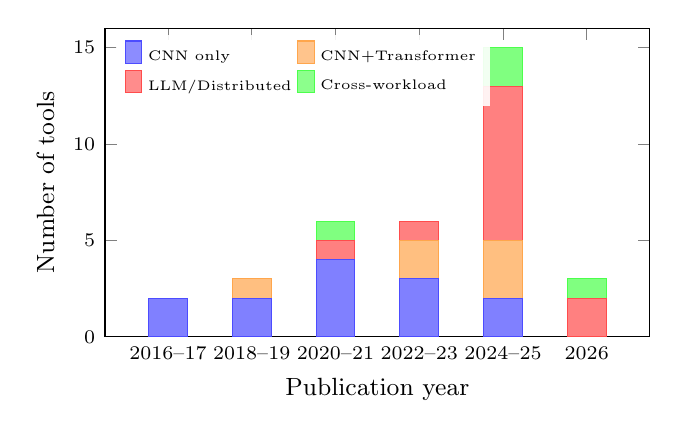
\begin{tikzpicture}
\begin{axis}[
    ybar stacked,
    bar width=14pt,
    xlabel={Publication year},
    ylabel={Number of tools},
    ymin=0, ymax=16,
    xtick={2016,2018,2020,2022,2024,2026},
    xticklabels={2016--17,2018--19,2020--21,2022--23,2024--25,2026},
    xticklabel style={font=\scriptsize},
    yticklabel style={font=\scriptsize},
    xlabel style={font=\small},
    ylabel style={font=\small},
    legend style={at={(0.02,0.98)}, anchor=north west, font=\tiny, draw=none, fill=white, fill opacity=0.9, text opacity=1, legend columns=2},
    legend cell align={left},
    height=5.5cm,
    width=8.5cm,
    enlarge x limits={abs=0.8cm},
]
\addplot[fill=blue!50, draw=blue!70] coordinates {(2016,2) (2018,2) (2020,4) (2022,3) (2024,2) (2026,0)};
\addplot[fill=orange!50, draw=orange!70] coordinates {(2016,0) (2018,1) (2020,0) (2022,2) (2024,3) (2026,0)};
\addplot[fill=red!50, draw=red!70] coordinates {(2016,0) (2018,0) (2020,1) (2022,1) (2024,8) (2026,2)};
\addplot[fill=green!50, draw=green!70] coordinates {(2016,0) (2018,0) (2020,1) (2022,0) (2024,2) (2026,1)};
\legend{CNN only, CNN+Transformer, LLM/Distributed, Cross-workload}
\end{axis}
\end{tikzpicture}%
}
\caption{Workload coverage of surveyed tools by publication period. The shift toward transformer and LLM workloads accelerates from 2023, but MoE and diffusion models remain largely uncharacterized.}
\label{fig:workload-coverage}
\end{figure}

\textbf{The composition problem.}
Composing kernel-level predictions into end-to-end estimates is unsolved: NeuSight's 2.3\% kernel MAPE yields $\sim$$10\times$ higher variance at model level ($\sigma_{\text{model}} \approx \sigma_{\text{kernel}} \cdot \sqrt{N}$), and correlated errors can compound linearly.
VIDUR sidesteps this by profiling entire prefill/decode phases.

\textbf{Emerging hardware and reproducibility.}
PIM architectures, chiplets, and disaggregated designs blur conventional memory hierarchy assumptions, while hardware-aware optimizations (FlashAttention~\cite{flashattention2022}) change the landscape faster than models can be retrained.
No equivalent of MLPerf~\cite{mlperf_training2020,mlperf_inference2020} exists for performance \emph{prediction}---standardized benchmarks would advance the field.
Analytical models remain the most interpretable, while ML-augmented approaches offer limited causal understanding.

\textbf{Future directions.}
Five priorities: (1)~transformer/MoE-aware tools with validated non-CNN accuracy; (2)~validated composition methods with bounded end-to-end error; (3)~unified energy-latency-memory prediction~\cite{mlperfpower2025}; (4)~temporal robustness benchmarks for software stack evolution; (5)~unified tooling with Docker-first deployment, portable formats (ONNX), and standard workload representations (Chakra~\cite{chakra2023}).

% ==============================================================================
% CONCLUSION
% ==============================================================================
\section{Conclusion}
\label{sec:conclusion}

This survey analyzed approximately 25 tools for predicting ML workload performance.
Key findings: methodology determines trade-offs (analytical: fast + interpretable; hybrid: best accuracy--speed balance at 2.3\% MAPE); LLM workloads demand purpose-built tools (VIDUR, Frontier); and Docker-first deployment is the strongest reproducibility predictor (8.5+/10 vs.\ 3/10 without).
The most pressing gaps are CNN-to-transformer generalization, kernel-to-end-to-end error composition, and emerging hardware support.

%%%%%%% -- PAPER CONTENT ENDS -- %%%%%%%%

%%
%% The next two lines define the bibliography style to be used, and
%% the bibliography file.
\bibliographystyle{ACM-Reference-Format}
\bibliography{references}

\end{document}
